\begin{surferPage}{卡萊三次曲面}
這個三次曲面當然也在簡單曲面的展覽之中。它共有四個錐形奇異點。19世紀亞瑟卡萊做過很多關於三次曲面的研究。這個三次曲面是以他的名字命名的。

然而,魯維格斯盲範系統地研究了曲面上奇異點的各種可能並在1863年第一次給出了這些曲面的分類。比如,他在文章中證明瞭三次曲面上的奇異點不會多於4個。這實際上是證明瞭$\mu(3)=4$.

大約在1900年,弗萊克斯克萊因研究實三次曲面的各種可能的形狀。他試圖用小形變的思想來回答產生於卡萊三次曲面的問題。通過擴張雙錐形奇異點,分裂或合併部分曲面,他成功地找到了所有三次曲面的形狀。下面
下面是其中的幾種:
 \vspace{0.3cm}
     \begin{center}
      \vspace{-0.2cm}
      \begin{tabular}{@{}c@{\ }c@{\ }c@{\ }c@{}}
        \begin{tabular}{@{}c@{}}
          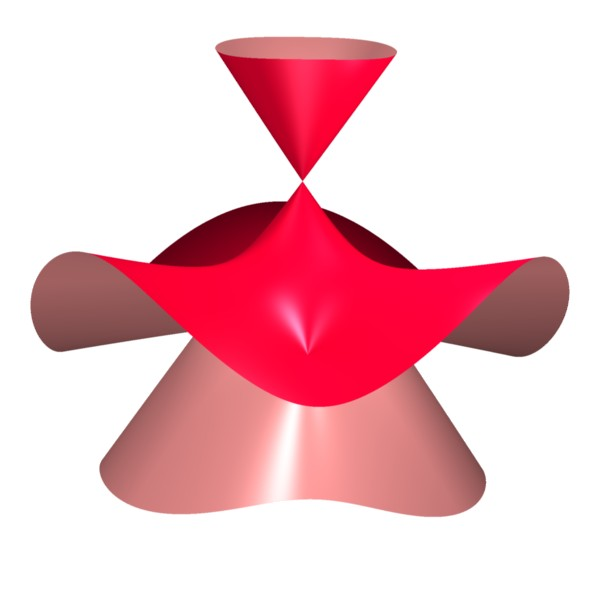
\includegraphics[width=1.35cm]{./../../common/images/cayley_cubic_0}
        \end{tabular}
        &
        \begin{tabular}{@{}c@{}}
          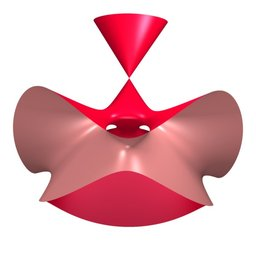
\includegraphics[width=1.35cm]{./../../common/images/cayley_cubic_1}
        \end{tabular}
        &
        \begin{tabular}{@{}c@{}}
          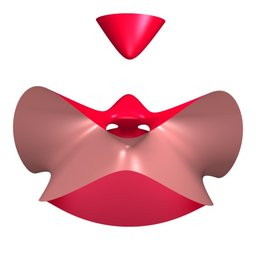
\includegraphics[width=1.35cm]{./../../common/images/cayley_cubic_2}
        \end{tabular}
        &
        \begin{tabular}{@{}c@{}}
          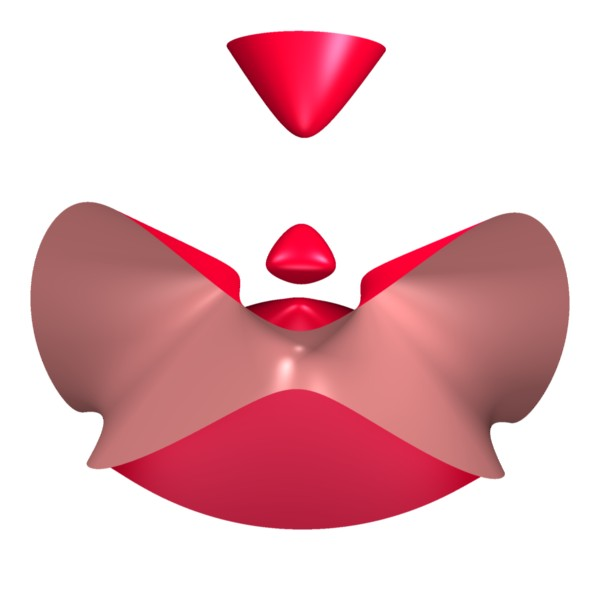
\includegraphics[width=1.35cm]{./../../common/images/cayley_cubic_3}
        \end{tabular}
      \end{tabular}
    \end{center}
\end{surferPage}
